%% 
%% Copyright 2007-2020 Elsevier Ltd
%% 
%% This file is part of the 'Elsarticle Bundle'.
%% ---------------------------------------------
%% 
%% It may be distributed under the conditions of the LaTeX Project Public
%% License, either version 1.2 of this license or (at your option) any
%% later version.  The latest version of this license is in
%%    http://www.latex-project.org/lppl.txt
%% and version 1.2 or later is part of all distributions of LaTeX
%% version 1999/12/01 or later.
%% 
%% The list of all files belonging to the 'Elsarticle Bundle' is
%% given in the file `manifest.txt'.
%% 
%% Template article for Elsevier's document class `elsarticle'
%% with harvard style bibliographic references

\documentclass[preprint,10pt,numbers]{elsarticle}

%% Use the option review to obtain double line spacing
%% \documentclass[authoryear,preprint,review,12pt]{elsarticle}

%% Use the options 1p,twocolumn; 3p; 3p,twocolumn; 5p; or 5p,twocolumn
%% for a journal layout:
%% \documentclass[final,1p,times,authoryear]{elsarticle}
%% \documentclass[final,1p,times,twocolumn,authoryear]{elsarticle}
%% \documentclass[final,3p,times,authoryear]{elsarticle}
%% \documentclass[final,3p,times,twocolumn,authoryear]{elsarticle}
%% \documentclass[final,5p,times,authoryear]{elsarticle}
%% \documentclass[final,5p,times,twocolumn,authoryear]{elsarticle}

% imports
\usepackage[margin=1in]{geometry}
\usepackage{amssymb}
\usepackage{amsmath}

% template package imports
\usepackage[utf8]{inputenc} % allow utf-8 input
\usepackage[T1]{fontenc}    % use 8-bit T1 fonts
\usepackage{xcolor}
\usepackage{hyperref}       % hyperlinks
\definecolor{BlueLink}{RGB}{15,78, 155}
\definecolor{lightgray}{gray}{0.9}
\hypersetup{
    colorlinks, allcolors=BlueLink
}

\usepackage{url}            % simple URL typesetting
\usepackage{booktabs}       % professional-quality tables
\usepackage{amsfonts}       % blackboard math symbols
\usepackage{nicefrac}       % compact symbols for 1/2, etc.
\usepackage{microtype}      % microtypography
\usepackage{cleveref}       % smart cross-referencing
\usepackage{lipsum}         % Can be removed after putting your text content
\usepackage{graphicx}
\usepackage{doi}
%\usepackage{mdframed}       % shaded figures
\usepackage{framed}      
\definecolor{shadecolor}{rgb}{0.95,0.95,0.95}

% my package imports
\usepackage{amssymb}
\usepackage{amsmath}
\usepackage{bm}       % bolding
\usepackage{stmaryrd} %jumps, avg
\usepackage{enumitem} %% removing whitespace for itemize
\usepackage{wrapfig}
\usepackage{subcaption}  
\usepackage{float} % table locations

%tunable policies imports
\usepackage{dsfont}
\usepackage{mathrsfs}
\usepackage{dirtytalk}

%\usepackage{floatrow}
% \usepackage[belowskip=-30pt,aboveskip=0pt]{caption}
\setlength{\textfloatsep}{8pt plus 1.0pt minus 2.0pt}
\setlength{\floatsep}{4pt plus 1.0pt minus 1.0pt}
\setlength{\intextsep}{5pt plus 1.0pt minus 1.0pt}
\setlength{\abovecaptionskip}{5pt plus 1pt minus 2pt}
% \captionsetup[figure]{font=small,skip=-100mm}

% graphics
\ifpdf
\DeclareGraphicsExtensions{.eps,.pdf,.png,.jpg}
\else
\DeclareGraphicsExtensions{.eps}
\fi 

% math general
%\newtheorem{lemma}{Lemma}
%\newtheorem{corollary}{Corollary}
%\newtheorem{proposition}{Proposition}
%\newtheorem{theorem}{Theorem}
%\theoremstyle{definition}
%\newtheorem{definition}{Definition}
%\newtheorem{remark}{Remark}

%\crefname{figure}{Figure}{Figs.}
%\crefname{chapter}{chapter}{chapters}
%\crefname{equation}{}{}
\DeclareMathOperator{\diag}{diag}
\newcommand{\nullspace}{{\mathcal N}}
\newcommand{\reals}{{\mbox{\bf R}}}
\newcommand{\ones}{\mathbf 1}

% domain, geometry
\newcommand{\Th}{\mathcal{T}_h}
\newcommand{\LII}{L^2}
\newcommand{\dom}{\Omega}
\newcommand{\bnd}{\partial\Omega}
\newcommand{\bndN}{\Gamma_{N}}
\newcommand{\bndD}{\Gamma_{D}}
\newcommand{\bndIn}{\Gamma_{\text{in}}}
\newcommand{\bndOut}{\Gamma_{\text{out}}}

% DG integrals, jumps, FEM ops
\newcommand{\Iint}[3]{\left(#1 ,\, #2 \right)_{#3}}
\newcommand{\IintK}[2]{\Iint{#1}{#2}{\gls{K}}}
\newcommand{\Eint}[3]{\left\langle #1 ,\, #2 \right\rangle_{#3}}
\newcommand{\EintK}[2]{\Eint{#1}{#2}{\partial K}}
\newcommand{\jmp}[1]{\llbracket #1 \rrbracket}
\newcommand{\mean}[1]{\left\{\!\left\{#1\right\}\!\right\}}
\newcommand{\nrml}{\hat{\mathbf n}}
\newcommand{\intk}[1]{\left(#1 \right)_K}
\newcommand{\intdk}[1]{\left \langle #1 \right \rangle_{\partial K}}

% variables
\newcommand{\vel}{\bm{u}}
\newcommand{\velh}{\bm{u}_h}
\newcommand{\p}{p}
\newcommand{\ph}{p_h}
\newcommand{\deltap}{\delta_{p}}
\newcommand{\dph}{\delta_{p,h}}
\newcommand{\qdph}{\bm{q}_{\delta_{p},h}}

% errors
\newcommand{\erroru}{\text{e}_{\velh}}
\newcommand{\errorp}{\text{e}_{\ph}}

% restriction operator, misc
\newcommand\restr[2]{{ % we make the whole thing an ordinary symbol
  \left.\kern-\nulldelimiterspace % automatically resize the bar with \right
  #1 % the function
  \vphantom{\big|} % pretend it's a little taller at normal size
  \right|_{#2} % this is the delimiter
  }}

% textual, English, annotation
\newcommand{\cf}{{\it cf.}}
\newcommand{\eg}{{\it e.g.}}
\newcommand{\ie}{{\it i.e.}}
\newcommand{\etc}{{\it etc.}}
\newcommand{\todo}[1]{{\color{blue}#1}}


%% The lineno packages adds line numbers. Start line numbering with
%% \begin{linenumbers}, end it with \end{linenumbers}. Or switch it on
%% for the whole article with \linenumbers.
%% \usepackage{lineno}

\journal{Journal of Computational Physics}

\begin{document}

\begin{frontmatter}

%% Title, authors and addresses

%% use the tnoteref command within \title for footnotes;
%% use the tnotetext command for theassociated footnote;
%% use the fnref command within \author or \affiliation for footnotes;
%% use the fntext command for theassociated footnote;
%% use the corref command within \author for corresponding author footnotes;
%% use the cortext command for theassociated footnote;
%% use the ead command for the email address,
%% and the form \ead[url] for the home page:
%% \title{Title\tnoteref{label1}}
%% \tnotetext[label1]{}
%% \author{Name\corref{cor1}\fnref{label2}}
%% \ead{email address}
%% \ead[url]{home page}
%% \fntext[label2]{}
%% \cortext[cor1]{}
%% \affiliation{organization={},
%%            addressline={}, 
%%            city={},
%%            postcode={}, 
%%            state={},
%%            country={}}
%% \fntext[label3]{}

\title{Projection methods for the incompressible Navier--Stokes equations using high-order hybridizable discontinuous Galerkin schemes}%

%% use optional labels to link authors explicitly to addresses:
%% \author[label1,label2]{}
%% \affiliation[label1]{organization={},
%%             addressline={},
%%             city={},
%%             postcode={},
%%             state={},
%%             country={}}
%%
%% \affiliation[label2]{organization={},
%%             addressline={},
%%             city={},
%%             postcode={},
%%             state={},
%%             country={}}

\author[MechE]{Corbin Foucart}
\ead{foucartc@mit.edu}
\author[MechE]{C. Mirabito}
\author[MechE]{P. J. Haley, Jr.}
\author[MechE]{Pierre F.J. Lermusiaux\corref{cor_author}}
\cortext[cor_author]{Corresponding author, }
\ead{pierrel@mit.edu}

\affiliation[MechE]{organization={Department of Mechanical Engineering, Computational Science and Engineering, Massachusetts Institute of Technology},
            addressline={77 Massachusetts Avenue}, 
            city={Cambridge},
            postcode={02139}, 
            state={MA},
            country={USA}}

\begin{abstract}
abstract.tex


\end{abstract}

\begin{keyword}
Nonhydrostatic modeling \sep
Finite element methods\sep
Discontinuous Galerkin methods
%% keywords here, in the form: keyword \sep keyword
%% PACS codes here, in the form: \PACS code \sep code
%% MSC codes here, in the form: \MSC code \sep code
%% or \MSC[2008] code \sep code (2000 is the default)
\end{keyword}

\end{frontmatter}

%\linenumbers


\section{Introduction}


In \cite{fehn_robust_2018}, the authors investigate the stability and robustness of DG discretizations of several projection methods. They compare fully-implicit, high-order dual splitting \cite{karniadakis_high-order_1991}, and pressure-correction schemes, but weirdly discretize the advection term implicitly for the pressure-correction, making the system nonlinear. So not exactly a fair comparison, since solving a nonlinear problem defeats the purpose of a projection method.

The numerical experiments in \cite{fehn_robust_2018} suggest that the high-order, dual splitting scheme 


\subsection{Incompressible Navier--Stokes}
\begin{equation}
  \begin{aligned}
  \frac{\partial \bm{u}}{\partial t} 
    + \nabla \cdot \left(\bm{u} \otimes \bm{u}\right) 
    - \nabla \cdot \left(\nu \nabla\bm{u}\right)
    + \nabla p = \bm{f} & \qquad \text{ on } \Omega \times [0,T] \\
    \nabla \cdot \bm{u} = 0 & \qquad  \text{ on } \Omega \times [0,T]
  \end{aligned}
  \label{eq:INS}
\end{equation}

Th incompressible Navier--stokes equations are subject to the initial condition
\begin{equation}
  \bm{u}(\bm{x},t=0) = \bm{u}_0 \text{ on } \Omega,
\end{equation}
where $\bm{u}_0$ is divergence-free. We denote the outward-facing unit normal vector as $\bm{n}$.  On the boundary $\Gamma$, we prescribe Dirichlet and Neumann conditions on $\Gamma_D$ and $\Gamma_N$, respectively, such that $\Gamma_D \cup \Gamma_N = \Gamma$.  
\begin{eqnarray}
  \bm{u} &= \bm{g}_D^u & \text{ on } \Gamma_D \times [0,T] \\ 
  \left(\bm{F}_v\left(\bm{u}\right) - p\bm{I}\right)\cdot\bm{n} &= \bm{g}_N^{\text{stress}} & \text{ on } \Gamma_D \times [0,T] 
\end{eqnarray}
Where $\bm{F}_v(\bm{u})$ is a representation of the viscous flux, usually given as $\bm{F}_v(\bm{u})=\nu \nabla \bm{u}$. The operator splitting associated with projection methods will necessitate splitting the boundary condition as well, so we decompose the stress condition into viscous and pressure components $\bm{g}_N^{\text{stress}} = \bm{g}_N^u - g_N^p\bm{n}$ and prescribe them separately, following \cite{fehn_robust_2018},
\begin{eqnarray}
  \bm{F}_v(\bm{u}) \cdot\bm{n} &= \bm{g}_N^u & \text{ on } \Gamma_N, \\
  p &= g_N^p & \text{ on } \Gamma_N.
\end{eqnarray}

We use the Rothe method, handling the temporal discretization and operator splitting before spatial discretization. For time integration, we apply backward differentiation formula (BDF) for all schemes in this paper.

\section{Projection methods}%

An overview of the temporal discretization and operator splitting for pressure-correction schemes is given in \cite{guermond_overview_2006}. Results from \cite{guermond_overview_2006}: (1) under certain smoothness requirements on the solution, the nonlinear advection term in the Navier--Stokes equations does not affect the convergence rates of the splitting errors, and they treat it explicitly. 

\subsubsection{Velocity predictor step}
An intermediate predictor velocity $\bar{\bm{u}}$ is calculated by solving the momentum equation with an explicit extrapolation of the pressure gradient term and explicit treatment of the advection term
\begin{equation}
\frac{ \beta_s \bar{\bm{u}} - \sum_{i=0}^{s_u-1}\left(\beta_i \bm{u}^{n-i}\right) }{\Delta t} 
- \nabla \cdot \left(\nu \nabla \bar{\bm{u}}\right) 
= - \sum_{i=0}^{s_p-1}\left(\gamma_i\nabla p^{n-i}\right) 
- \nabla \cdot \left(\bm{u}^n\otimes \bm{u}^n\right) 
+ \bm{f}(t_{n+1}),
\label{eq:PDE_velocity_predictor}
\end{equation}
where the boundary conditions for the predictor velocity are 
\begin{align}
  \begin{aligned}
  \bar{\bm{u}} &= \bm{g}_D^u(t_{n+1}) & \text{ on } \Gamma_D, \\
  \left(\nu \nabla \bar{\bm{u}}\right) \cdot \bm{n} &= \bm{g}_N^u(t_{n+1}) & \text{ on } \Gamma_N.
  \end{aligned}
  \label{eq:VP_BCs}
\end{align}

\subsubsection{Pressure corrector step}
The second step involves computing a correction $\delta p^{k+1}$ to the pressure by solving 
\begin{equation}
  -\nabla^2 \delta p^{k+1} = - \frac{\beta_s}{\Delta t} \nabla \cdot \bar{\bm{u}},
  \label{eq:PC_presure_poisson}
\end{equation}
subject to the boundary conditions
\begin{eqnarray}
    \nabla \delta p^{n+1} \cdot \bm{n} = 0 & \text{ on } \Gamma_D, \\
    \delta p^{n+1} = g_p(t_{n+1}) 
    - \sum_{i=0}^{s_p-1}\left(\beta_i g_p(t_{n-i})\right) & \text{ on }  \Gamma_N.
\label{eq:PDE_pressure_corrector}
\end{eqnarray}

The pressure Poisson equation (\ref{eq:PC_presure_poisson}) is obtained by
writing the intermediate velocity $\bar{\bm{u}}$ in terms of a Helmholtz
decomposition consisting of a solenoidal component $\bm{u}$ (since $\nabla \cdot
\bm{u}= 0$) and irrotational component $\nabla \delta p^{n+1}$,
\begin{eqnarray}
  \frac{\beta_s}{\Delta t} \bm{u}^{n+1} + \nabla \delta p^{n+1} =
  \frac{\beta_s}{\Delta t} \bar{\bm{u}}, \label{eq:PC:helmholtz} \\
  \delta p^{n+1} = p^{n+1} 
    - \sum_{i=0}^{s_p-1}\left(\beta_i p^{n-i}\right) 
    + \chi \nu \nabla \cdot \bar{\bm{u}},
\end{eqnarray}
then taking the divergence of equation (\ref{eq:PC:helmholtz}), making use of the divergence-free constraint $\nabla \cdot \bm{u}^{n+1} = 0 $. Taking $\chi=0$ corresponds to the standard formulation and $\chi=1$ the rotational formulation of the method, respectively \cite{guermond_overview_2006}. We consider the rotational formulation hereafter.  

\subsubsection{Projection step}
In the third step, the velocity $\bm{u}^{n+1}$ and pressure $p^{n+1}$ at time $t_{n+1}$ are obtained by performing updates amounting to the projection of $\bar{\bm{u}}$ onto the space of divergence-free vector fields

\begin{align}
  \bm{u}^{n+1} &= \bar{\bm{u}} - \frac{\Delta t}{\beta_s} \nabla \delta p^{n+1}, \\
  p^{n+1} &= \sum_{i=0}^{s_p-1} \left(\beta_i p^{n-i}\right) 
  + \delta p^{n+1} 
  - \nu \nabla \cdot \bar{\bm{u}},
\end{align}

Theoretical rates of convergence for the pressure-corrector schemes are given in \cite{guermond_overview_2006}.
The authors suggest that schemes are only conditionally stable for $s_p \geq 2$.
To ensure unconditional stability, we therefore select $s_u = 2$ and $s_p = 1$.
With these choices, the pressure-corrector scheme using the rotational formulation can be expected to be $\Delta t^2$ accurate in the $L^2$-norm of the velocity and $\Delta t^{3/2}$ accurate in the $L^2$-norm of the pressure.


\section{Spatial discretization}

\subsection{Notation}
Boilerplate

\subsection{Finite element spaces}
boilerplate

\subsection{HDG Pressure-correction scheme}

The choice of spatial discretization for the pressure gradient terms and the velocity divergence term is of central importance to the stability and robustness of the projection schemes in \cite{fehn_robust_2018}. Previous work in \cite{ueckermann_lermusiaux_JCP2016} conducted limited investigation of the discretization of these terms as they appeared in HDG discretizations of projection methods. This motivates the present work in determining whether the discretization of these two terms is similarly important to the robustness of HDG schemes. 

The point of departure for HDG schemes is to write each semi-discretized PDE as a first-order system, which we do for the velocity predictor equation (\ref{eq:PDE_velocity_predictor})  and pressure correction equation (\ref{eq:PDE_pressure_corrector}). The projection step does not require an implicit formulation and is computed directly.

\subsubsection{HDG formulation of explicit operators}

\textit{Pressure gradient terms}. The pressure gradient term can 
We integrate by parts and replace $p_h$ on the element boundary $\partial K$ with a central numerical flux $p^*_h = \mean{p_h} $. Applying the mean operator definitions on the interior and boundary interfaces separately,
\begin{equation}
  \text{pg}_h(\bm{v}, p_h, g_N^p) = -\left(\nabla \cdot \bm{v},\, p_h \right)_{\Th} 
  + \left\langle \bm{v},\mean{p_h}\bm{n}\right\rangle_{\partial\Th \setminus \Gamma}
  + \left\langle \bm{v}, g_N^p\bm{n}\right\rangle_{\Gamma_N}
  + \left\langle \bm{v}, p_h\bm{n}\right\rangle_{\Gamma_D}
\end{equation}%
As in Fehn et al., we consider also an alternate reference formulation used in \cite{hesthaven_nodal_2008,ueckermann_lermusiaux_JCP2016}, which does not integrate the pressure gradient by parts,
\begin{equation}
  \text{pg}_{h,\text{ref}}(\bm{v}, p_h) = \left(\bm{v},\, \nabla p_h \right)_{\Th} 
\end{equation}

\textit{Advection term}. The advection term
\begin{equation}
  F_a(\bm{v}, \bm{u}_h)
\end{equation}

\textit{Velocity divergence term}. The HDG formulation of the velocity divergence term pertains to the discretization of terms of the form $\left(w,\, \nabla \cdot \bar{\bm{u}}_h \right)_K$ over an element $K$. Just as for the pressure gradient term, we integrate by parts and replace $\bm{u}_h$ on the element boundary $\partial K$ with a central numerical flux $\bar{\bm{u}}^*_h = \mean{\bar{\bm{u}}_h} $. Applying the mean operator definitions on the interior and boundary interfaces separately,
\begin{equation}
\text{vd}_h(w,\bar{\bm{u}}_h, \bm{g}_D^u)  =  (\nabla w,\, \bar{\bm{u}}_h)_{\mathcal{T}_h}
 + \langle w,\, \mean{\bar{\bm{u}}_h} \cdot\bm{n}\rangle_{\partial\mathcal{T}_h\setminus \Gamma}
 + \langle w,\, \bar{\bm{u}}_h \cdot\bm{n}\rangle_{\Gamma_N}
 + \langle w,\, \bm{g}_D^u \cdot\bm{n}\rangle_{\Gamma_D}
 ,
\end{equation}
where we could have taken $\bm{g}_D^u = \bar{\bm{u}}_h$ instead, since this is enforced in equation (\ref{eq:VP_BCs}). Just as for the pressure gradient term, we consider also an alternate reference formulation given in \cite{hesthaven_nodal_2008}, 
\begin{equation}
  \text{vd}_{h,\text{ref}}(w,\bar{\bm{u}}_h) = \left(w, \nabla \cdot \bar{\bm{u}}_h \right)_{\Th},
\end{equation}
which does not perform integration by parts. 

note: in \cite{ueckermann_lermusiaux_JCP2016}, We integrate by parts another time (equivalent) but take $\widehat{\bar{\bm{u}}}_h^{k+1}$ as the HDG flux from the predictor solve, which may be unsound.

In addition to the form of the terms themselves, HDG methods provide different choices of numerical flux which we have to investigate. Using the HDG fluxes themselves as numerical fluxes for these terms turns out to require quite complicated accounting in order to make sure the scheme stays consistent. Since the HDG flux is in some sense an intermediate quantity designed to allow for static condensation and reduction of globally-coupled degrees of freedom, it makes more sense to avoid using these fluxes elsewhere in the time discretization. Further, storing the fluxes incurs additional memory costs and requires correction \cite{ueckermann_lermusiaux_JCP2016}.

\subsubsection{Velocity predictor}%
Rewritten as a first-order system, equation (\ref{eq:PDE_velocity_predictor}) takes the form
\begin{equation}
  \begin{aligned}
    \bar{\bm{L}} - \nabla \bm{u} &= 0  \\
    \frac{ \beta_s \bar{\bm{u}} - \sum_{i=0}^{s_u-1}\left(\beta_i \bm{u}^{n-i}\right) }{\Delta t} 
    - \nabla \cdot \left(\nu \bar{\bm{L}}\right) 
    &= - \sum_{i=0}^{s_p-1}\left(\gamma_i\nabla p^{n-i}\right) 
    - \nabla \cdot \left(\bm{u}^n\otimes \bm{u}^n\right) 
    + \bm{f}(t_{n+1}),
  \end{aligned}
  \label{eq:velocity_predictor_first_order}
\end{equation}
where the first equation defines a new tensor-valued unknown $\bar{\bm{L}}$ approximating the velocity gradient $\nabla\bar{\bm{u}}$, and the second is equation (\ref{eq:PDE_velocity_predictor}) written in terms of $\bar{\bm{L}}$.
Taking the numerical flux definition $\left(-\nu \hat{\bm{\bar{L}}}_h \right)\bm{n} \equiv \left(-\nu \bm{\bar{L}}_h\right)\bm{n} + \tau (\bm{\bar{u}}_h - \hat{\bm{u}}_h)$ and adding an equation to weakly enforce the continuity of its normal component on the space $M_h^p$ \cite{nguyen_hybridizable_2010,nguyen_implicit_2011}, we arrive at the following weak form

The velocity predictor $\bar{\bm{u}}_h$
\begin{equation}
  \begin{aligned}
    ( \bm{G} ,\, \bm{\bar{L}}_h)_{\Th} 
    + ( \nabla \cdot \bm{G} ,\, \bm{\bar{u}}_h)_{\Th} 
   - \langle \bm{G}\cdot\bm{n} ,\, \hat{\bm{u}}_h \rangle_{\partial \Th} &=0 \\
   \left( \bm{v} ,\, \frac{\beta_s}{\Delta t} \bar{\bm{u}} \right)_{\Th}
    - \left( \bm{v} ,\, \nabla \cdot  \left(\nu \bm{\bar{L}}_h\right) \right)_{\Th}
    + \langle \bm{v} ,\, \tau \left(\bm{\bar{u}}_h - \hat{\bm{u}}_h\right) \rangle_{\partial \Th}
    &= \left(\bm{v},\,  \sum_{i=0}^{s_u-1}\left(\frac{\beta_i}{\Delta t}  \bm{u}^{n-i}\right) \right)_{\Th} \\
     - \sum_{i=0}^{s_p-1}\left(\gamma_i\,\text{pg}_h(\bm{v}, p_h^{n-i},g^p_N(t_{n-i}))\right) 
    &+ F_a(\bm{v},\bm{u}_h)
    + (\bm{v},\, \bm{f})_{\Th} \\
    \left\langle \bm{\mu} ,\, (-\nu \bar{\bm{L}}_h)\bm{n} + \tau(\bar{\bm{u}}_h - \hat{\bm{u}}_h) \right\rangle_{\partial \mathcal{T}_h \setminus \Gamma_D} 
+ \left\langle \bm{\mu} ,\, \widehat{b}_h \right\rangle_{\Gamma_N} &= 0
  \end{aligned}
\end{equation}
This differs from the scheme in \cite{ueckermann_lermusiaux_JCP2016}, which takes the jump of the pressure in the numerical flux.

This admits a matrix-discretization over each element:
\begin{equation}
  \begin{bmatrix}
   A   &  B & -C \\
   B^T &  -D & E \\
   -N & G &  -H
  \end{bmatrix}
  \begin{bmatrix} L_h \\ U_h \\ \widehat{U}_h \end{bmatrix}
  =
  \begin{bmatrix} 0 \\ -(F - P) \\ -L \end{bmatrix}.
\end{equation}

In the case where the velocity components are not coupled on the boundary of the mesh due to the boundary conditions, for example, when a zero Dirichlet no-slip condition is applied to the velocity along a non-trivial bathymetry, and the vertical sides of the domain are axis-aligned, the linear system arising from equation (\ref{eq:coupled_velocity_predictor_weak_form}) is decoupled, and the predictor velocity can be solved component-by-component.

Let $\bar{\phi}$ represent any component of the velocity $\bar{\bm{u}}$.
If we were to write the usual form of the HDG problem where $\bm{q} = \nu \nabla\bar{\phi}$ represents the complete gradient of the component $\bar{\phi}$, then we want to find $(\bar{\phi}, \bm{q})\in W_h\times \bm{V}_h$ such that 
\begin{equation}
  \begin{aligned}
    \left(\bm{v},\, \nu^{-1}\bm{q}\right)_{\Th} 
    +\left(\nabla \cdot \bm{v},\, \bar{\phi} \right)_{\Th}
    - \left\langle \bm{v}\cdot\bm{n},\, \hat{\phi} \right\rangle_{\partial\Th} &=0\\
    \left(w,\, \frac{\bar{\phi}}{a \Delta t} \right)_{\Th}
    + \left(w,\, \nabla \cdot \left( \bm{q}\right) \right)_{\Th}
    - \left\langle w,\, \tau\left(\bar{\phi}-\hat{\phi}\right) \right\rangle_{\partial\Th} 
    &= \text{rh}_h(w,\bm{u}^k,p_h^k, \bm{F})_K \\
    \left\langle \mu,\, \widehat{\bm{q}}\cdot\bm{n} \right\rangle_{\partial\Th} &= \left\langle \mu,\, g_N \right\rangle_{\Gamma_N}
  \end{aligned}
\end{equation}
where the operator $\text{rh}_h(\cdot)$ contains all the component-wise right-hand side terms of the momentum equation. 
This formulation is consistent with the full 3D velocity predictor if $\nu_{xy}=\nu_z$. 
This also couples the domain together on the interfaces.
The velocity predictor $\bm{\bar{u}}_h^{k+1}$ is the vector $(\bar{\phi}_u,\, \bar{\phi}_v,\, \bar{\phi}_w)$ resulting from each of the HDG solves.

In the decoupled case, the formulation of the DG right-hand side operators can be obtained by considering only the relevant component $w$ of the test function $\bm{v}\in \bm{V}_h^p$ as appears in equation (\ref{eq:coupled_velocity_predictor_weak_form}). 
For the advective term, we have 
\begin{equation}
  a_h(w,\bar{\phi}, \bm{u}_h^k, \bm{g}_D) 
  = -\left(w,\, \nabla \cdot \left( \bar{\phi}\bm{u}_h^k \right)\right)_K
   = - \left(\nabla w,\, \bar{\phi}\bm{u}^k_h\right)_K
   + \left\langle w, \left(\bar{\phi}\bm{u}_h^k\right)^* \cdot\bm{n} \right\rangle_{\partial K},
\end{equation}
where the operator $a_h(\cdot)$ can be be treated explicitly by taking $\bar{\phi} = u^k_{h,j}$ where the integer $j$ denotes the spatial dimension corresponding to the component of the predictor velocity sought, or it can be treated semi-implicitly (\cf  \,\cite{nguyen_implicit_2009}) as written; in the latter case, the weak form is no longer symmetric.
In this paper, we consider a completely explicit treatment.
\todo{need to consider boundary treatment for the advective flux--compare table in Fehn with naive approach!}
The numerical flux in this work $\left(\bar{\phi}\bm{u}_h^k\right)^*$ is taken to be an upwind flux.
Since $\bm{u}_h^k$ is multiply-valued, either the average value $\mean{\bm{u}_h}$ or the HDG flux $\hat{\bm{u}}_h$ can be used.

Similarly, the pressure gradient term for the component $i$ of $\bar{\bm{u}}_h^{k+1}$, $\bar{\phi}_i$, is
\begin{equation}
  \text{pg}_h\left(w,p_h^k\right) = 
    - \left(\frac{\partial w}{\partial x_i},\, p^{\prime,k}_h\right)
    + \left\langle w,\, \left(p^{\prime, k}_h\right)^*n_i \right\rangle
\end{equation}
where $n_i$ denotes the $i^{\text{th}}$ component of the outward unit normal $\bm{n}$, and where the numerical flux is again chosen to be the central flux, $\left(p^{\prime, k}_h\right)^* = \mean{p_h^{\prime,k}}$.

\subsubsection{Pressure corrector}%
The weak form for the pressure corrector can be expressed as 
\begin{equation}
\begin{aligned}
(\bm{v},\,  \bm{q}_{\delta p}^{k+1})_{\mathcal{T}_h}
+ ( \nabla \cdot \bm{v} ,\, \delta p^{k+1})_{\mathcal{T}_h}
- \langle \bm{v}\cdot\bm{n} ,\, \widehat{\delta p} \rangle_{\partial \mathcal{T}_h} &= 0 \\
-(w ,\, \nabla \cdot \bm{q}_{\delta p}^{k+1})_{\mathcal{T}_h}
+ \langle w,\, \tau_p \delta p^{k+1}\rangle_{\partial \mathcal{T}_h} 
- \langle w,\, \tau_p \widehat{\delta p} \rangle_{\partial \mathcal{T}_h} 
&= - \frac{\beta_s}{\Delta t} \text{vd}_h(w,\bar{\bm{u}}_h, \bm{g}_D^u(t_{n+1}))  \\
\left\langle \mu ,\, \bm{q}_{\delta p}^{k+1} \cdot\bm{n} + \tau_p(\delta p^{k+1} - \widehat{\delta p})
\right\rangle_{\partial \mathcal{T}_h \setminus \Gamma_D} &= 0 
\end{aligned}
\end{equation}

\subsection{Inhomogeneous boundary condition treatment}
\subsection{Numerical flux definitions}

\section{Numerical experiments}
\label{sec:numerical_experiments}

\subsection{Implementation}%
\label{sec:implementation_details}

The finite element forward models were implemented in \texttt{C++} and make use of the finite element library \texttt{deal.ii} \cite{dealII93}.

\todo{
All surface and volume integral operators are discretized with Gaussian quadrature using $p_{\text{order}}+1$ one-dimensional (1D) quadrature points in each spatial direction, where $p_{\text{order}}$ is the polynomial order of the finite element space (space)}. 
%$W_h^\porder$.

Convergence results are reported using the relative $L^2$-errors 
\begin{equation}
  \erroru(t) = \frac{ \left\lVert \vel(\bm{x}, t) - \velh(\bm{x}, t)\right\rVert_{\LII(\dom_h)} }{ \left\lVert \vel(\bm{x}, t) \right\rVert_{\LII(\dom_h)} }, \qquad 
  \errorp(t) =\frac{ \left\lVert \p(\bm{x}, t) - \ph(\bm{x}, t)\right\rVert_{\LII(\dom_h)} }{ \left\lVert \p(\bm{x}, t) \right\rVert_{\LII(\dom_h)} },
\end{equation}
where each of the $\LII$-norms over the computational domain $\dom_h$ is calculated using Gaussian quadrature over the element volumes using $p_{\bm{u}} + 3$ for errors in the velocity and $p_{p} + 3$ for errors in the pressure variables.
Unless explicitly specified, the abbreviations $\erroru$ and $\errorp$ refer to the velocity and pressure errors at the final time $T$.


\subsection{On the solution of the pure Neumann problem}

In the case of pure Dirichlet boundaries on the velocity predictor, the pressure level is undefined. 
To see this, note that if the scalar field $\delta p_h$ is a solution of (\ref{eq:PC_presure_poisson}) with $\Gamma_N = \partial \Omega$, then $\delta p_h + c$ for any $c \in \reals$ is also a solution. 
Discretely, the null space of the linear system arising due to the discretization of (\ref{eq:PC_presure_poisson}) is spanned by the set of constant vectors, implying a singular linear system.


Although crucial to the performance of pressure correction schemes, the issue of finding a solution to the singular system in such cases receives little attention in the literature. 
iterative solvers \cite{axelsson_iterative_1996,iankov_finite_2013}, 
An approach favored by many practitioners is to manually specify the value of the candidate solution at a single point by removing an equation from the discrete system and applying a Dirichlet constraint fixing the value of the solution at that point to an arbitrary constant, eliminating the null space and allowing solution of the linear system using a conventional direct solver.
However, in a finite-element context, the function $\delta_p$ is often represented in the Sobolev space $H^1(\Omega)$ or $L^2(\Omega)$, spaces in which point evaluations do not make sense. 
In these cases, imposing such a constraint can render the variational problem ill-posed.

\todo{
This is complicated by the fact that some numerical linear algebra software varies widely in terms of implementation; while some libraries will not solve a singular system (numpy), other direct procedures will do so when they can identify a zero-pivot. 
Similar for iterative solvers.}


In \cite{bochev_finite_2005}, the authors rigorously describe strategies for addressing the singular system in a continuous finite element context. 
Here, we extend that discussion to the DG-FEM setting and illustrate computational trade-offs associated with some candidate approaches.

As a first approach, we apply a subspace projection using a Krylov-solver \cite{vorst_iterative_2003}, making use of the fact that iterative solvers solve singular systems provided that the right-hand side is in the orthogonal complement of the null-space.
\todo{
This modification is ok because we're only removing the null space contribution to the linear system
}
As a second approach, we apply a penalty-based method which can be interpreted as a regularization.
This method, while simple and independent of linear solver type, involves the specification of a hyperparameter $\gamma$.
As a third approach, we impose a mean-value constraint 
\begin{equation}
  \int_{\Omega}^{} \delta p \,d\Omega = 0
  \label{eq:mean_value_zero_condition}
\end{equation}
into the linear system directly, avoiding the saddle point system that arises as a result of applying the constraint as a Lagrange multiplier \cite{bochev_finite_2005}.

\todo{
As a test case, we use a manufactured solution
How to do the zero-mean removal?
}

Boundary conditions and forcing function are deduced from the exact solution
\begin{equation}
    \delta_p^* = \frac{1}{3} \sin\left(-\frac{\pi}{2} x \right) \cos\left(2\pi y\right).
\end{equation}
We consider the domain $\Omega = [-1, 1]^2$, and by symmetry, we have that the exact solution $\delta_p^*$ is analytically zero-mean in the sense of equation (\ref{eq:mean_value_zero_condition}).

\begin{figure}[htpb]
  \centering
  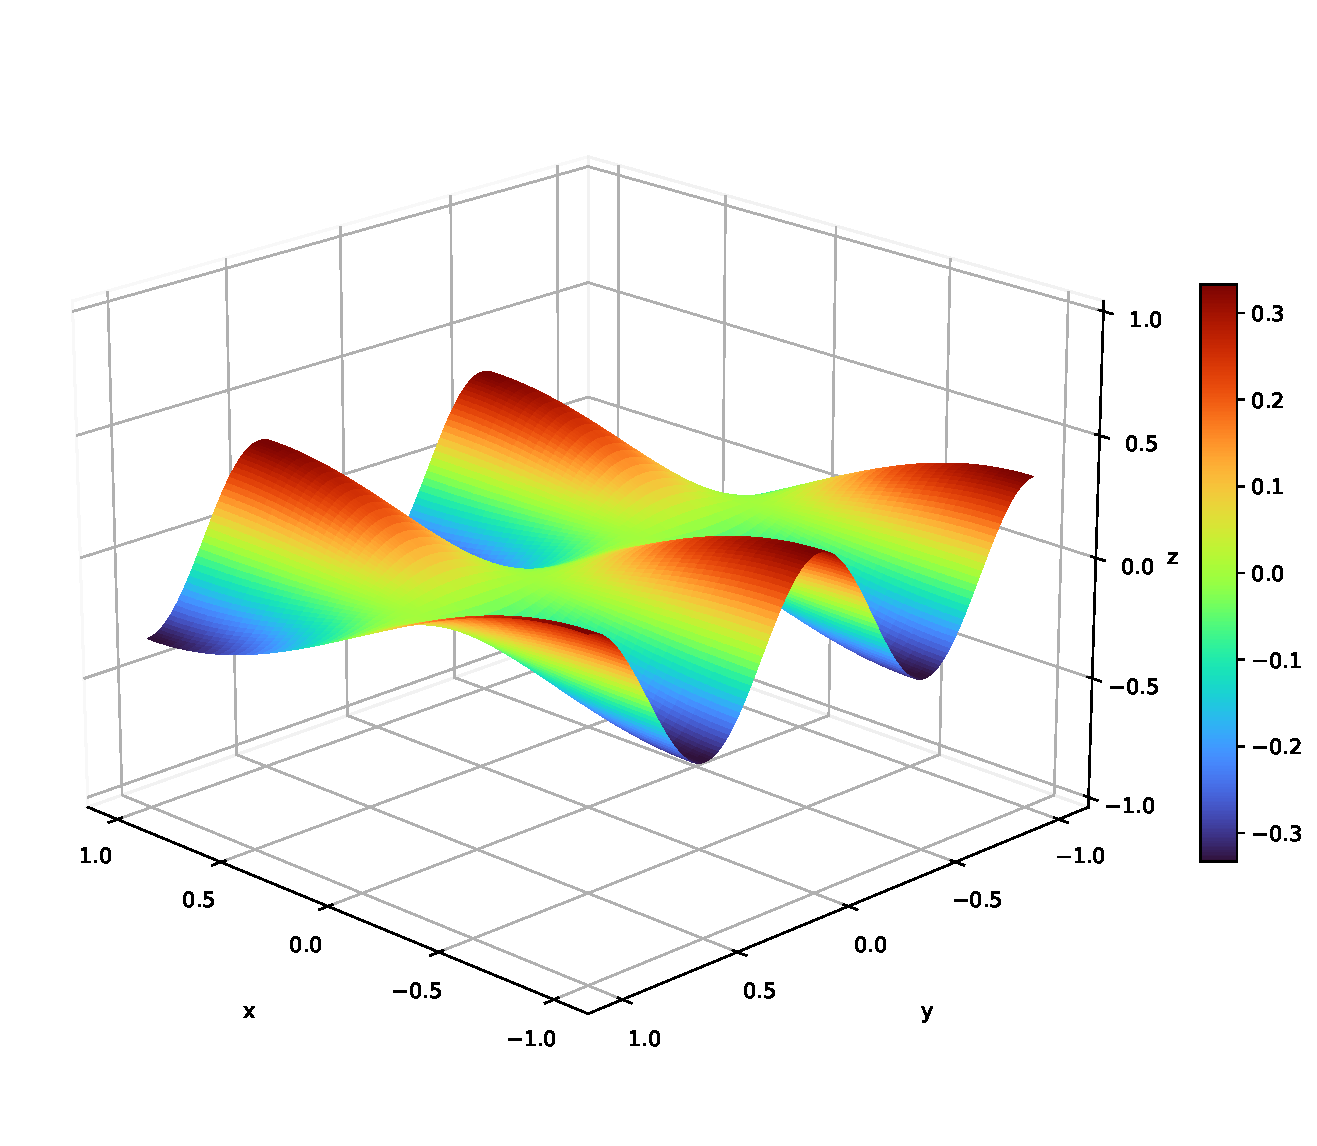
\includegraphics[width=0.5\linewidth]{img/dp_study_analytical.pdf}
  \caption{Analytical solution of the pure Neumann problem}
  \label{fig:dp_neumann_problem_analytical}
\end{figure}




\subsection{Unsteady Stokes Flow}

The review paper \cite{guermond_overview_2006} solves the unsteady Stokes problem

\begin{equation}
  \begin{aligned}
    \bm{u}(\bm{x}, t) &= \pi \sin t 
    \begin{pmatrix}
      \sin( 2\pi y) \sin^2( \pi x) \\
      -\sin(2 \pi x) \sin^2(\pi y)
    \end{pmatrix} \\
    p(\bm{x}, t) &= \sin(t)\cos(\pi x) \sin(\pi y)\\
  \end{aligned}
  \label{eq:MS_stokes_guermond}
\end{equation}
where the source term $f= u_t -\nu \nabla \cdot( \nabla \bm{u} ) + \nabla p $.

In \cite{fehn_stability_2017}, we have
\begin{equation}
  \begin{aligned}
  \bm{u}(\bm{x}, t) &= 
  \begin{pmatrix}
    \sin(x) (a\sin(a y) - \cos(a)\sinh(y)) \\
    \cos(x) (\cos(a y) + \cos(a)\cosh(y))
  \end{pmatrix}
  \exp(-\lambda t),\\
    p(\bm{x}, t) &= \lambda \cos(a) \cos(x) \sinh(y) \exp(-\lambda t)
  \end{aligned}
  \label{eq:MS_unsteady_stokes_fehn}
\end{equation}
where $\lambda = \nu(1 + a^2)$ $\nu = 1$ and $a = 2.883356$ on a domain of  $\Omega = [-1, 1]^2$; they take $[0, T] = [0, 0.1]$ and Dirichlet boundary conditions everywhere, $\Gamma = \Gamma_D$.

\subsection{Verification}
Spatial convergence test, temporal convergence test




\subsection{Taylor-Green vortex flow}
Is this the same test case as in Hesthaven?

\subsection{Backward facing step}

\subsection{Lid-driven cavity flow}

\subsection{Lock Exchange?}
\subsection{Lab RTI flow?}



\section{Discussion}%

The imposition of open boundary conditions where inflow and outflow can co-exist remains an open problem in the finite element community \cite{sani_resume_1994}. 

\section{Appendix: BDF1}%
\label{sec:appendix_bdf1}


%%


%%Vancouver style references.
%\bibliographystyle{model1-num-names}
%\bibliographystyle{alpha} %[Axe96]
\bibliographystyle{abbrv} % [1]

{\footnotesize
\bibliography{mseas,FEM}
}

\end{document}

%% main text
